% Options for packages loaded elsewhere
\PassOptionsToPackage{unicode}{hyperref}
\PassOptionsToPackage{hyphens}{url}
\PassOptionsToPackage{dvipsnames,svgnames,x11names}{xcolor}
%
\documentclass[
]{article}

\usepackage{amsmath,amssymb}
\usepackage{iftex}
\ifPDFTeX
  \usepackage[T1]{fontenc}
  \usepackage[utf8]{inputenc}
  \usepackage{textcomp} % provide euro and other symbols
\else % if luatex or xetex
  \usepackage{unicode-math}
  \defaultfontfeatures{Scale=MatchLowercase}
  \defaultfontfeatures[\rmfamily]{Ligatures=TeX,Scale=1}
\fi
\usepackage{lmodern}
\ifPDFTeX\else  
    % xetex/luatex font selection
\fi
% Use upquote if available, for straight quotes in verbatim environments
\IfFileExists{upquote.sty}{\usepackage{upquote}}{}
\IfFileExists{microtype.sty}{% use microtype if available
  \usepackage[]{microtype}
  \UseMicrotypeSet[protrusion]{basicmath} % disable protrusion for tt fonts
}{}
\makeatletter
\@ifundefined{KOMAClassName}{% if non-KOMA class
  \IfFileExists{parskip.sty}{%
    \usepackage{parskip}
  }{% else
    \setlength{\parindent}{0pt}
    \setlength{\parskip}{6pt plus 2pt minus 1pt}}
}{% if KOMA class
  \KOMAoptions{parskip=half}}
\makeatother
\usepackage{xcolor}
\usepackage[top=30mm,left=20mm,heightrounded]{geometry}
\setlength{\emergencystretch}{3em} % prevent overfull lines
\setcounter{secnumdepth}{5}
% Make \paragraph and \subparagraph free-standing
\ifx\paragraph\undefined\else
  \let\oldparagraph\paragraph
  \renewcommand{\paragraph}[1]{\oldparagraph{#1}\mbox{}}
\fi
\ifx\subparagraph\undefined\else
  \let\oldsubparagraph\subparagraph
  \renewcommand{\subparagraph}[1]{\oldsubparagraph{#1}\mbox{}}
\fi


\providecommand{\tightlist}{%
  \setlength{\itemsep}{0pt}\setlength{\parskip}{0pt}}\usepackage{longtable,booktabs,array}
\usepackage{calc} % for calculating minipage widths
% Correct order of tables after \paragraph or \subparagraph
\usepackage{etoolbox}
\makeatletter
\patchcmd\longtable{\par}{\if@noskipsec\mbox{}\fi\par}{}{}
\makeatother
% Allow footnotes in longtable head/foot
\IfFileExists{footnotehyper.sty}{\usepackage{footnotehyper}}{\usepackage{footnote}}
\makesavenoteenv{longtable}
\usepackage{graphicx}
\makeatletter
\def\maxwidth{\ifdim\Gin@nat@width>\linewidth\linewidth\else\Gin@nat@width\fi}
\def\maxheight{\ifdim\Gin@nat@height>\textheight\textheight\else\Gin@nat@height\fi}
\makeatother
% Scale images if necessary, so that they will not overflow the page
% margins by default, and it is still possible to overwrite the defaults
% using explicit options in \includegraphics[width, height, ...]{}
\setkeys{Gin}{width=\maxwidth,height=\maxheight,keepaspectratio}
% Set default figure placement to htbp
\makeatletter
\def\fps@figure{htbp}
\makeatother
\newlength{\cslhangindent}
\setlength{\cslhangindent}{1.5em}
\newlength{\csllabelwidth}
\setlength{\csllabelwidth}{3em}
\newlength{\cslentryspacingunit} % times entry-spacing
\setlength{\cslentryspacingunit}{\parskip}
\newenvironment{CSLReferences}[2] % #1 hanging-ident, #2 entry spacing
 {% don't indent paragraphs
  \setlength{\parindent}{0pt}
  % turn on hanging indent if param 1 is 1
  \ifodd #1
  \let\oldpar\par
  \def\par{\hangindent=\cslhangindent\oldpar}
  \fi
  % set entry spacing
  \setlength{\parskip}{#2\cslentryspacingunit}
 }%
 {}
\usepackage{calc}
\newcommand{\CSLBlock}[1]{#1\hfill\break}
\newcommand{\CSLLeftMargin}[1]{\parbox[t]{\csllabelwidth}{#1}}
\newcommand{\CSLRightInline}[1]{\parbox[t]{\linewidth - \csllabelwidth}{#1}\break}
\newcommand{\CSLIndent}[1]{\hspace{\cslhangindent}#1}

\usepackage{booktabs}
\usepackage{longtable}
\usepackage{array}
\usepackage{multirow}
\usepackage{wrapfig}
\usepackage{float}
\usepackage{colortbl}
\usepackage{pdflscape}
\usepackage{tabu}
\usepackage{threeparttable}
\usepackage{threeparttablex}
\usepackage[normalem]{ulem}
\usepackage{makecell}
\usepackage{xcolor}
\usepackage{siunitx}

  \newcolumntype{d}{S[
    input-open-uncertainty=,
    input-close-uncertainty=,
    parse-numbers = false,
    table-align-text-pre=false,
    table-align-text-post=false
  ]}
  
\makeatletter
\makeatother
\makeatletter
\makeatother
\makeatletter
\@ifpackageloaded{caption}{}{\usepackage{caption}}
\AtBeginDocument{%
\ifdefined\contentsname
  \renewcommand*\contentsname{Table of contents}
\else
  \newcommand\contentsname{Table of contents}
\fi
\ifdefined\listfigurename
  \renewcommand*\listfigurename{List of Figures}
\else
  \newcommand\listfigurename{List of Figures}
\fi
\ifdefined\listtablename
  \renewcommand*\listtablename{List of Tables}
\else
  \newcommand\listtablename{List of Tables}
\fi
\ifdefined\figurename
  \renewcommand*\figurename{Figure}
\else
  \newcommand\figurename{Figure}
\fi
\ifdefined\tablename
  \renewcommand*\tablename{Table}
\else
  \newcommand\tablename{Table}
\fi
}
\@ifpackageloaded{float}{}{\usepackage{float}}
\floatstyle{ruled}
\@ifundefined{c@chapter}{\newfloat{codelisting}{h}{lop}}{\newfloat{codelisting}{h}{lop}[chapter]}
\floatname{codelisting}{Listing}
\newcommand*\listoflistings{\listof{codelisting}{List of Listings}}
\makeatother
\makeatletter
\@ifpackageloaded{caption}{}{\usepackage{caption}}
\@ifpackageloaded{subcaption}{}{\usepackage{subcaption}}
\makeatother
\makeatletter
\@ifpackageloaded{tcolorbox}{}{\usepackage[skins,breakable]{tcolorbox}}
\makeatother
\makeatletter
\@ifundefined{shadecolor}{\definecolor{shadecolor}{rgb}{.97, .97, .97}}
\makeatother
\makeatletter
\makeatother
\makeatletter
\makeatother
\ifLuaTeX
  \usepackage{selnolig}  % disable illegal ligatures
\fi
\IfFileExists{bookmark.sty}{\usepackage{bookmark}}{\usepackage{hyperref}}
\IfFileExists{xurl.sty}{\usepackage{xurl}}{} % add URL line breaks if available
\urlstyle{same} % disable monospaced font for URLs
\hypersetup{
  pdftitle={The Unintended Consequences of Energy Reduction},
  pdfauthor={Yi Fei Pang; Irene Hyunh; Tara Chakkithara},
  colorlinks=true,
  linkcolor={blue},
  filecolor={Maroon},
  citecolor={Blue},
  urlcolor={Blue},
  pdfcreator={LaTeX via pandoc}}

\title{The Unintended Consequences of Energy Reduction\thanks{Code and
data are available at: LINK.}}
\usepackage{etoolbox}
\makeatletter
\providecommand{\subtitle}[1]{% add subtitle to \maketitle
  \apptocmd{\@title}{\par {\large #1 \par}}{}{}
}
\makeatother
\subtitle{How an Act of Environmental Protection Led to the Deaths of
Many}
\author{Yi Fei Pang \and Irene Hyunh \and Tara Chakkithara}
\date{February 13, 2024}

\begin{document}
\maketitle
\begin{abstract}
First sentence. Second sentence. Third sentence. Fourth sentence.
\end{abstract}
\ifdefined\Shaded\renewenvironment{Shaded}{\begin{tcolorbox}[breakable, interior hidden, frame hidden, enhanced, borderline west={3pt}{0pt}{shadecolor}, boxrule=0pt, sharp corners]}{\end{tcolorbox}}\fi

\hypertarget{introduction}{%
\section{Introduction}\label{introduction}}

\begin{figure}

{\centering 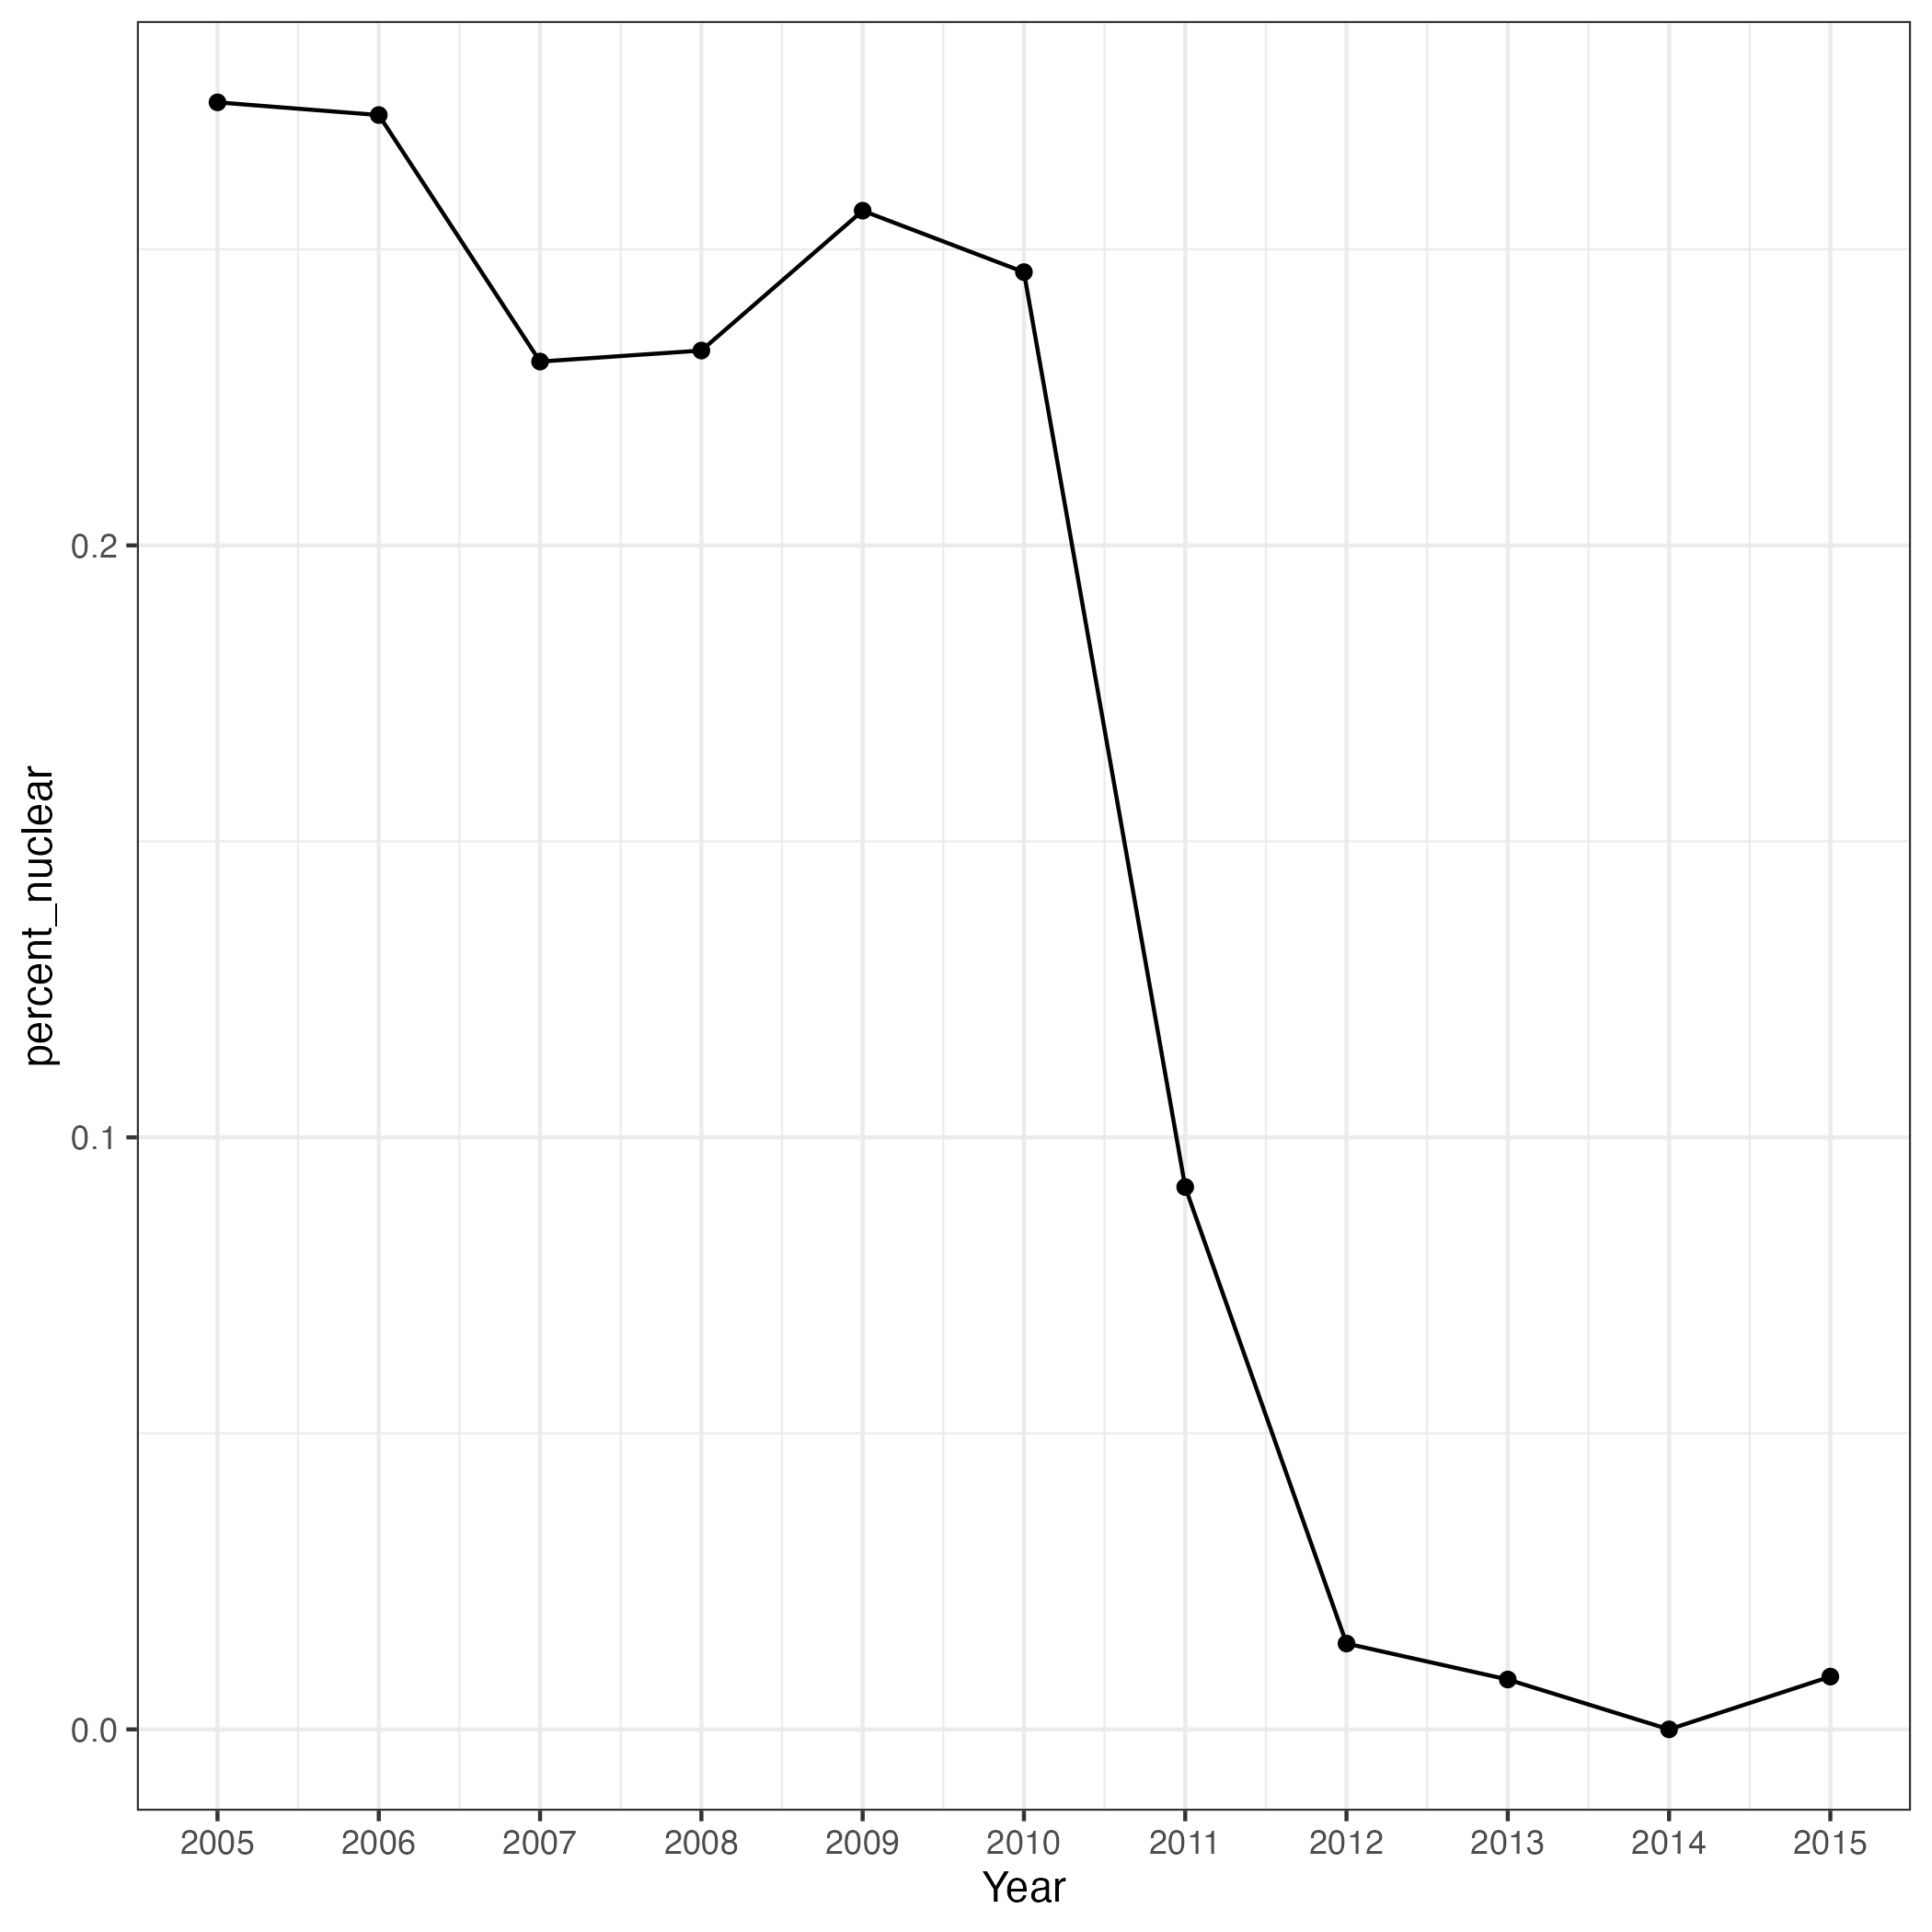
\includegraphics{../other/figures/figure1.png}

}

\caption{Figure 1}

\end{figure}

The 2011 Fukushima disaster changed the relationship Japanese citizens
had with nuclear energy. From the 160, 000 Fukushima residents that had
to evacuate the city to the citizens who may not have been affected
directly, the public as a whole turned their backs against the entire
industry {[}science direct{]}.

Before the accident, nuclear energy made up 25\% of Japan's energy
market. After the accident, the market share stayed under 1.7\% until
2016. The Democratic Party of Japan itself took initiative and
implemented a new energy policy to ``phase out nuclear power,''
{[}intchopen{]} despite formerly having close ties to the industry in
attempts to reduce CO2 pollution. {[}enpolicy one year later{]}

Fossil fuels grew to dominate Japan's energy market as many reactors
were shut down. In 2011 itself, oil usage rose by around 85\% while
natural gas increased by 25\%. {[}enpolicy one year later{]}

This change had a huge impact on the price and consumption of
electricity. Relative to the mean price of electricity in 2011, by 2013
the price of electricity had increased to over 10\% and almost reached
an increase of 20\% by 2014. Concurrently, electricity consumption
itself kept decreasing year after year as it became less affordable.
{[}figure 1{]}

A good reason for this market shift is that most of the fossil fuels
that Japan utilizes are exported from other countries, which makes them
expensive. {[}enpolicy one year later{]} The lack of nuclear power also
reduced more affordable options for consumers.

The trend of increasing electricity prices and decreasing electricity
consumption may persist into the future. The current government of Japan
reversed the nuclear energy policy, but low public demand for nuclear
energy still persists. Thus the prices will stay high as people continue
to consume fossil fuels. There are also barriers to nuclear power that
help to persist this trend. One barrier is the Nuclear Regulation
Authority which created tougher safety regulations for reactors. Another
are injunctions that citizens can bring forth to prevent the operation
of nuclear reactors. After the Fukushima tragedy many courts in Japan
may grant these injunctions for safety reasons. {[}intchopen{]}

You can and should cross-reference sections and sub-sections. We use R
Core Team (2023) and Wickham et al. (2019).

The remainder of this paper is structured as follows.
Section~\ref{sec-data}\ldots.

\hypertarget{sec-data}{%
\section{Data}\label{sec-data}}

Some of our data is of penguins (\textbf{?@fig-bills}), from Horst,
Hill, and Gorman (2020).

Talk more about it.

And also planes (\textbf{?@fig-planes}). (You can change the height and
width, but don't worry about doing that until you have finished every
other aspect of the paper - Quarto will try to make it look nice and the
defaults usually work well once you have enough text.)

Talk way more about it.

\hypertarget{model}{%
\section{Model}\label{model}}

The goal of our modelling strategy is twofold. Firstly,\ldots{}

Here we briefly describe the Bayesian analysis model used to
investigate\ldots{} Background details and diagnostics are included in
Appendix~\ref{sec-model-details}.

\hypertarget{results}{%
\section{Results}\label{results}}

Our results are summarized in \textbf{?@tbl-modelresults}.

\hypertarget{discussion}{%
\section{Discussion}\label{discussion}}

\hypertarget{sec-first-point}{%
\subsection{First discussion point}\label{sec-first-point}}

\hypertarget{second-discussion-point}{%
\subsection{Second discussion point}\label{second-discussion-point}}

\hypertarget{third-discussion-point}{%
\subsection{Third discussion point}\label{third-discussion-point}}

\hypertarget{weaknesses-and-next-steps}{%
\subsection{Weaknesses and next steps}\label{weaknesses-and-next-steps}}

A few weaknesses with the analysis comes from the limitation of data.The
scope of analysis for the post-Fukushima incident and the effects of the
energy policy is only Japan. There is no comparison to other countries
and their markets trends after nuclear accidents such as Ukraine with
the Chernobyl incident. Furthermore, the data is limited only from the
Fukushima incident up until 2016 allowing for a short term analysis. The
physical effects of nuclear incidents along with the economic effects of
the energy policy are both issues that can use a more long term
approach. Additionally, there is a lack of robustness as the analysis is
fixated on the effects caused by the transition from nuclear energy to
fossil fuels. However, there are other energy sources such as renewable
energy which includes solar and wind energy that should be taken into
consideration.

The next steps would be to find more recent data. As aforementioned, the
datasets only extend until 2016 and to complete a long-term analysis,
more recent Japanese energy data needs to be collected. Moreover, data
from before and after other global nuclear incidents should be gathered
and evalauted in comparison to Fukushima to evaluate whether the
Japanese government's apporoach was the most optimal. Another step that
can be taken to futher the analysis could be to explore more granular
effects. For example, in addition to looking at how temperatures and
strokes can be correlated (pls verify we did this?), other factors such
as energy price variation and seasons or energy jobs and employment
rates can be observed as well.

\newpage

\appendix

\hypertarget{appendix}{%
\section*{Appendix}\label{appendix}}
\addcontentsline{toc}{section}{Appendix}

\hypertarget{additional-data-details}{%
\section{Additional data details}\label{additional-data-details}}

\hypertarget{sec-model-details}{%
\section{Model details}\label{sec-model-details}}

\hypertarget{posterior-predictive-check}{%
\subsection{Posterior predictive
check}\label{posterior-predictive-check}}

In \textbf{?@fig-ppcheckandposteriorvsprior-1} we implement a posterior
predictive check. This shows\ldots{}

In \textbf{?@fig-ppcheckandposteriorvsprior-2} we compare the posterior
with the prior. This shows\ldots{}

\hypertarget{diagnostics}{%
\subsection{Diagnostics}\label{diagnostics}}

\textbf{?@fig-stanareyouokay-1} is a trace plot. It shows\ldots{} This
suggests\ldots{}

\textbf{?@fig-stanareyouokay-2} is a Rhat plot. It shows\ldots{} This
suggests\ldots{}

\newpage

\hypertarget{references}{%
\section*{References}\label{references}}
\addcontentsline{toc}{section}{References}

\hypertarget{refs}{}
\begin{CSLReferences}{1}{0}
\leavevmode\vadjust pre{\hypertarget{ref-palmerpenguins}{}}%
Horst, Allison Marie, Alison Presmanes Hill, and Kristen B Gorman. 2020.
\emph{Palmerpenguins: Palmer Archipelago (Antarctica) Penguin Data}.
\url{https://doi.org/10.5281/zenodo.3960218}.

\leavevmode\vadjust pre{\hypertarget{ref-citeR}{}}%
R Core Team. 2023. \emph{R: A Language and Environment for Statistical
Computing}. Vienna, Austria: R Foundation for Statistical Computing.
\url{https://www.R-project.org/}.

\leavevmode\vadjust pre{\hypertarget{ref-rohan}{}}%
Wickham, Hadley, Mara Averick, Jennifer Bryan, Winston Chang, Lucy
D'Agostino McGowan, Romain François, Garrett Grolemund, et al. 2019.
{``Welcome to the {tidyverse}.''} \emph{Journal of Open Source Software}
4 (43): 1686. \url{https://doi.org/10.21105/joss.01686}.

\end{CSLReferences}



\end{document}
